
\let\negmedspace\undefined
\let\negthickspace\undefined
\documentclass[journal,12pt,twocolumn]{IEEEtran}
%\documentclass[conference]{IEEEtran}
%\IEEEoverridecommandlockouts
% The preceding line is only needed to identify funding in the first footnote. If that is unneeded, please comment it out.
\usepackage{cite} %support for author-year citations 
\usepackage{amsmath,amssymb,amsfonts,amsthm}
\usepackage{algorithmic}
\usepackage{caption}
\usepackage{graphicx}
\usepackage{textcomp} %text symbols, such as the degree symbol,currency,etc
\usepackage{xcolor} %colored text and background colors
\usepackage{txfonts} %e fonts are designed to be used in mathematical expressions, and include characters such as the Greek alphabet, mathematical symbols, and operators
\usepackage{multirow}
%\usepackage{enumitem} %customizing the appearance of lists.
\usepackage{mathtools} %exp,eqn,subscript,superscript
\usepackage{gensymb} %scientific symbols
\usepackage[breaklinks=true]{hyperref} %This package provides support for hyperlinks within a LaTeX document, including clickable references and URLs. 
%The breaklinks=true option tells LaTeX to break long URLs that would otherwise extend beyond the right margin of the page. This can help to improve the readability of the document, as it avoids the need to scroll horizontally to read long URLs.

\usepackage{tkz-euclide} % loads  TikZ and tkz-base
%tools for drawing geometric figures in a LaTeX document, with a focus on Euclidean geometry

\usepackage{listings} %The listings package can be used to display code from various programming languages, including C, C++, Java, Python, and many others. It also provides options to customize the appearance of the listings, such as changing the font, background color, line numbers, and more.
%
%\usepackage{setspace}  %commands to control the line spacing
%\usepackage{gensymb} 
%\doublespacing
%\singlespacing
%\usepackage{graphicx} %to include graphics (images) 
%\usepackage{amssymb} %additional mathematical symbols and fonts \subset, \supset, \in, \exists, \forall, \not\equiv, etc.
% example for real numberset \mathbb{R} 
%\usepackage{relsize} %provides a simple way to adjust the font size of math mode symbols and text in a flexible way. It provides the \mathlarger and \mathsmaller commands to adjust the size of math mode symbols and the \larger and \smaller commands to adjust the size of text
%\usepackage[cmex10]{amsmath}
%\usepackage{amsthm}
%\interdisplaylinepenalty=2500
%\savesymbol{iint}
%\usepackage{txfonts}
%\restoresymbol{TXF}{iint}
%\usepackage{wasysym}
\usepackage{amsthm}
\usepackage{amsmath}
%\usepackage{iithtlc}
%\usepackage{mathrsfs}
%\usepackage{txfonts}
%\usepackage{stfloats}
%\usepackage{bm}
%\usepackage{cite}
%\usepackage{cases}
%\usepackage{subfig}
%\usepackage{xtab}
%\usepackage{longtable}
%\usepackage{multirow}
%\usepackage{algorithm}
%\usepackage{algpseudocode}
%\usepackage{enumitem}
%\usepackage{mathtools}
%\usepackage{tikz}
%\usepackage{circuitikz}
%\usepackage{verbatim}
%\usepackage{tfrupee}
%\usepackage{stmaryrd}
%\usetkzobj{all}
%    \usepackage{color}                                            %%
%    \usepackage{array}                                            %%
%    \usepackage{longtable}                                        %%
%    \usepackage{calc}                                             %%
%    \usepackage{multirow}                                         %%
%    \usepackage{hhline}                                           %%
%    \usepackage{ifthen}                                           %%
  %optionally (for landscape tables embedded in another document): %%
%    \usepackage{lscape}     
%\usepackage{multicol}
%\usepackage{chngcntr}
%\usepackage{enumerate}

%\usepackage{wasysym}
%\newcounter{MYtempeqncnt}
%\DeclareMathOperator*{\Res}{Res}
%\renewcommand{\baselinestretch}{2}
%\renewcommand\thesection{\arabic{section}}
\renewcommand\thesection{\Roman{section}}
\renewcommand\thesubsection{\thesection.\Roman{subsection}}
%\renewcommand\thesubsection{\thesection.\arabic{subsection}}
%\renewcommand\thesubsubsection{\thesubsection.\arabic{subsubsection}}

\renewcommand\thesectiondis{\arabic{section}}
\renewcommand\thesubsectiondis{\thesectiondis.\arabic{subsection}}
\renewcommand\thesubsubsectiondis{\thesubsectiondis.\arabic{subsubsection}}

% correct bad hyphenation here
\hyphenation{op-tical net-works semi-conduc-tor}
\def\inputGnumericTable{}                                 %%

\lstset{
%language=C,
frame=single, 
breaklines=true,
columns=fullflexible
}

\begin{document}
%


\newcommand{\BEQA}{\begin{eqnarray}}
\newcommand{\EEQA}{\end{eqnarray}}
\newcommand{\define}{\stackrel{\triangle}{=}}

\bibliographystyle{IEEEtran}
%\bibliographystyle{ieeetr}


\providecommand{\mbf}{\mathbf}
\providecommand{\pr}[1]{\ensuremath{\Pr\left(#1\right)}}
\providecommand{\qfunc}[1]{\ensuremath{Q\left(#1\right)}}
\providecommand{\sbrak}[1]{\ensuremath{{}\left[#1\right]}}
\providecommand{\lsbrak}[1]{\ensuremath{{}\left[#1\right.}}
\providecommand{\rsbrak}[1]{\ensuremath{{}\left.#1\right]}}
\providecommand{\brak}[1]{\ensuremath{\left(#1\right)}}
\providecommand{\lbrak}[1]{\ensuremath{\left(#1\right.}}
\providecommand{\rbrak}[1]{\ensuremath{\left.#1\right)}}
\providecommand{\cbrak}[1]{\ensuremath{\left\{#1\right\}}}
\providecommand{\lcbrak}[1]{\ensuremath{\left\{#1\right.}}
\providecommand{\rcbrak}[1]{\ensuremath{\left.#1\right\}}}
\theoremstyle{remark}
\newtheorem{rem}{Remark}
\newcommand{\sgn}{\mathop{\mathrm{sgn}}}
\providecommand{\abs}[1]{\left\vert#1\right\vert}
\providecommand{\res}[1]{\Res\displaylimits_{#1}} 
\providecommand{\norm}[1]{\left\lVert#1\right\rVert}
%\providecommand{\norm}[1]{\lVert#1\rVert}
\providecommand{\mtx}[1]{\mathbf{#1}}
\providecommand{\mean}[1]{E\left[ #1 \right]}
\providecommand{\fourier}{\overset{\mathcal{F}}{ \rightleftharpoons}}
%\providecommand{\hilbert}{\overset{\mathcal{H}}{ \rightleftharpoons}}
\providecommand{\system}{\overset{\mathcal{H}}{ \longleftrightarrow}}
	%\newcommand{\solution}[2]{\textbf{Solution:}{#1}}
\newcommand{\solution}{\noindent \textbf{Solution: }}
\newcommand{\cosec}{\,\text{cosec}\,}
\providecommand{\dec}[2]{\ensuremath{\overset{#1}{\underset{#2}{\gtrless}}}}
\newcommand{\myvec}[1]{\ensuremath{\begin{pmatrix}#1\end{pmatrix}}}
\newcommand{\mydet}[1]{\ensuremath{\begin{vmatrix}#1\end{vmatrix}}}
%\numberwithin{equation}{section}
%\numberwithin{equation}{subsection}
%\numberwithin{problem}{section}
%\numberwithin{definition}{section}
%\makeatletter
%\@addtoreset{figure}{problem}
%\makeatother

%\let\StandardTheFigure\thefigure
\let\vec\mathbf

\vspace{3cm}

\title{
Report on Software Assignment\\Playing Audio Files Randomly\\AI1110 : Probability and Random Variables
}
\author{Tumarada Padmaja\\CS22BTECH11059}

% make the title area
\maketitle
%\newpage
\bigskip
\section{INTRODUCTION} 	The goal of assignment is to create a playlist of audiofiles and play them randomly. A program is written in Python using libraries like random,os and pygame libraries.
\\
\\
\section{CREATION OF AUDIO FILES FROM VIDEO FILES} The videos files provided have .mov extension which are converted into audio files using VLC media player i.e to .mp3 extension. A folder of these files is created.
\\
\\
\section{PLAYING THE AUDIO FILES RANDOMLY} The OS module in python is used to go through the files in the directory mentioned. Then a list called playlist is created using these files. Random module provides function random.shuffle which helps in shuffling the audio files in the playlist created i.e randomising it.
The pygame module is used for handling audio,multimedia applications,etc. This is used in the program to handle the audio files i.e to play, pause,resume,etc.
\\
\\
\section{FEATURES} The program asks user input for different purposes. \\
\textbf{Pause:} user can pause the audio by pressing \textbf{p}, this is achieved using the function pygame.mixer.music.pause()\\
\textbf{Resume:} user can resume the audio by pressing \textbf{r}, this is achieved using the function pygame.mixer.music.unpause()\\
\textbf{Next:} user can navigate to the next audio file by pressing \textbf{n}\\
\textbf{Quit } user can quit the audio by pressing \textbf{q}
\\
\\
\section{DESCRIPTION OF CODE } There are three loops used in main function.\\
One is an infinite while loop which is used here to resume the program until user wants to quit.\\
The next, for loop is used to iterate through and play the randomised playlist.\\
The inner while loop ensures that user is given opportunity to give input as long as a song is playing.\\
Other functions are to create a playlist, randomise it and play the audio files.
\\
\\
\section{OUTPUT} 
\begin{figure}[h]
  \centering
  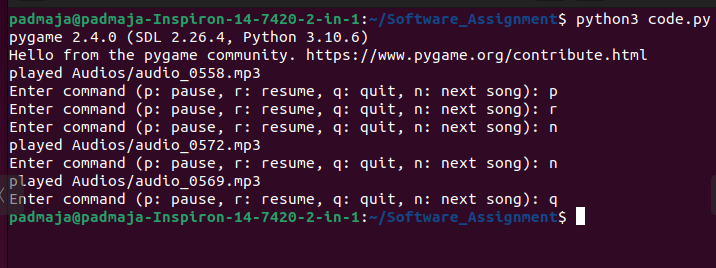
\includegraphics[bb=0 0 716 268,width=0.55\textwidth]{output.png}
  \captionsetup{justification=centering}
  \caption{User Interface}
\end{figure}
\section{CONCLUSION } Overall, the code produces a random playlist, keeps on generating until user asks to stop it. The flow of playlist is in the hands of user as at each step user is asked an input. A random playlist of MP3 files is created
and can be played by the user.


\end{document}


